
On consid\`ere le probl\`eme de contr\^ole optimal \eqref{eq:ocpBangReg}. L'objectif est de retrouver les r\'esultats des figures
\ref{fig:results_tests_continuation_1} et \ref{fig:results_tests_continuation} et de d\'eterminer la structure de la solution lorsque $\veps \to 0$.

\begin{figure}[ht!]
    \begin{center}
        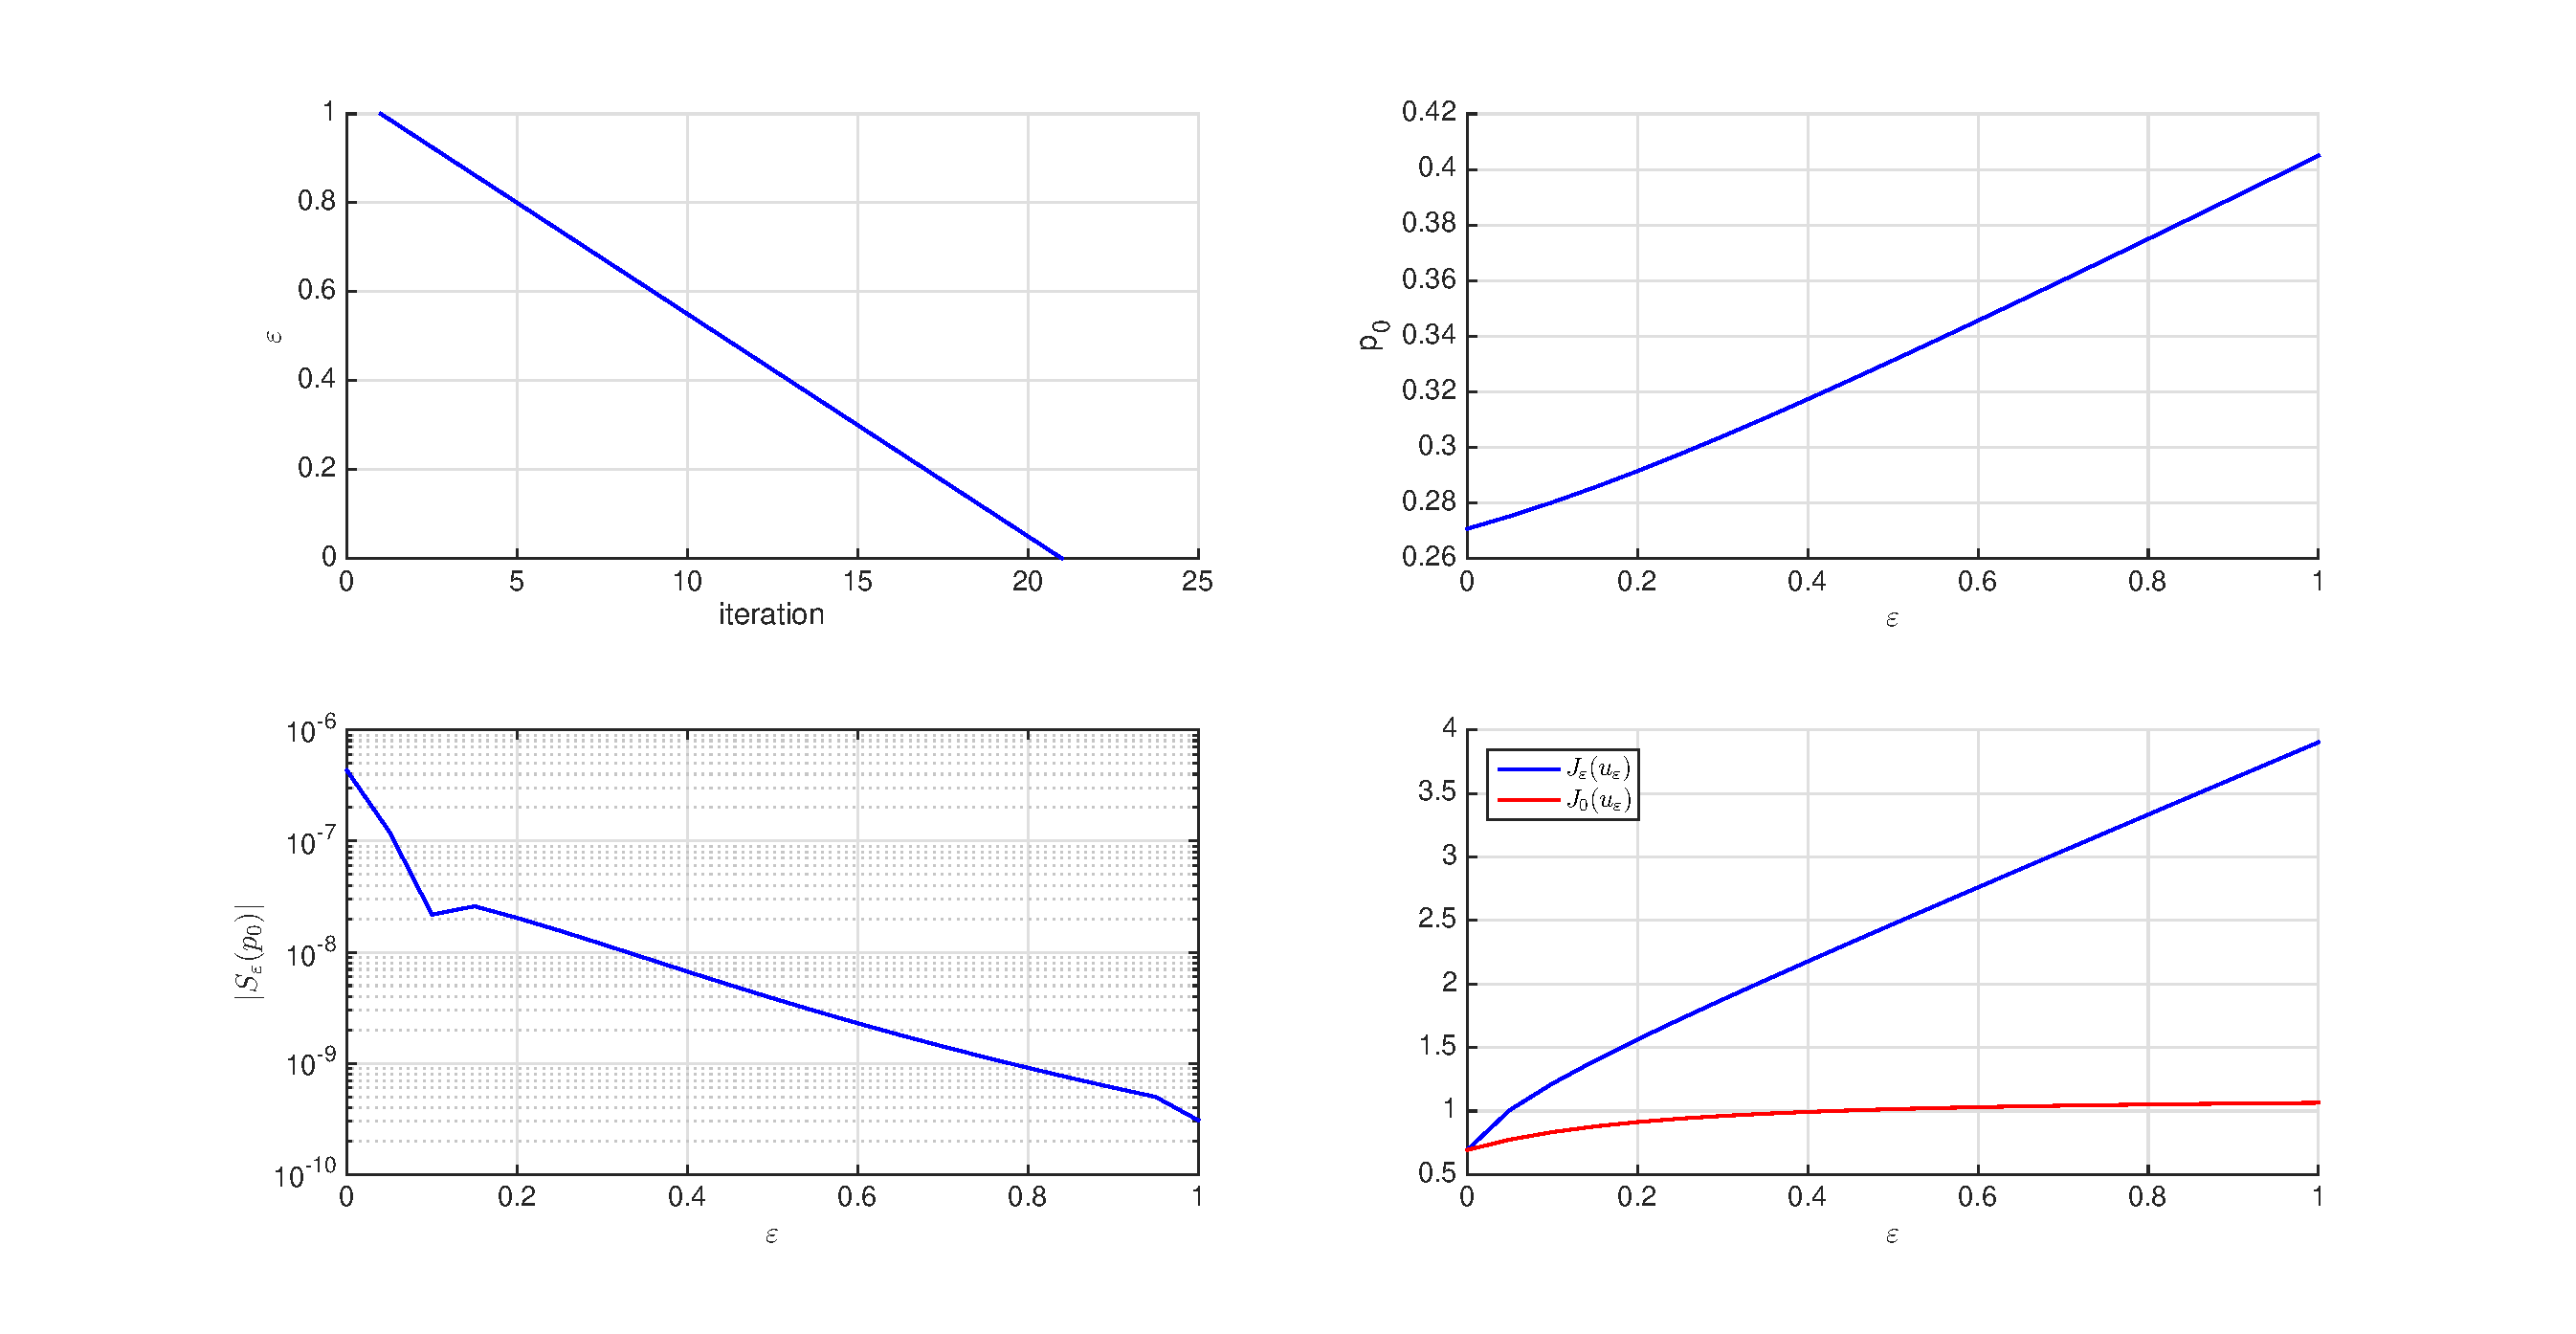
\includegraphics[width=0.99\textwidth]{results_tests_continuation_1}
    \end{center}
    \vspace{-3em}
    \caption{Figure 1 apr\`es ex\'ecution du fichier \cmd{sujet3\_continuation/main.m}.}
    \label{fig:results_tests_continuation_1}
\end{figure}

\begin{figure}[ht!]
    \begin{center}
        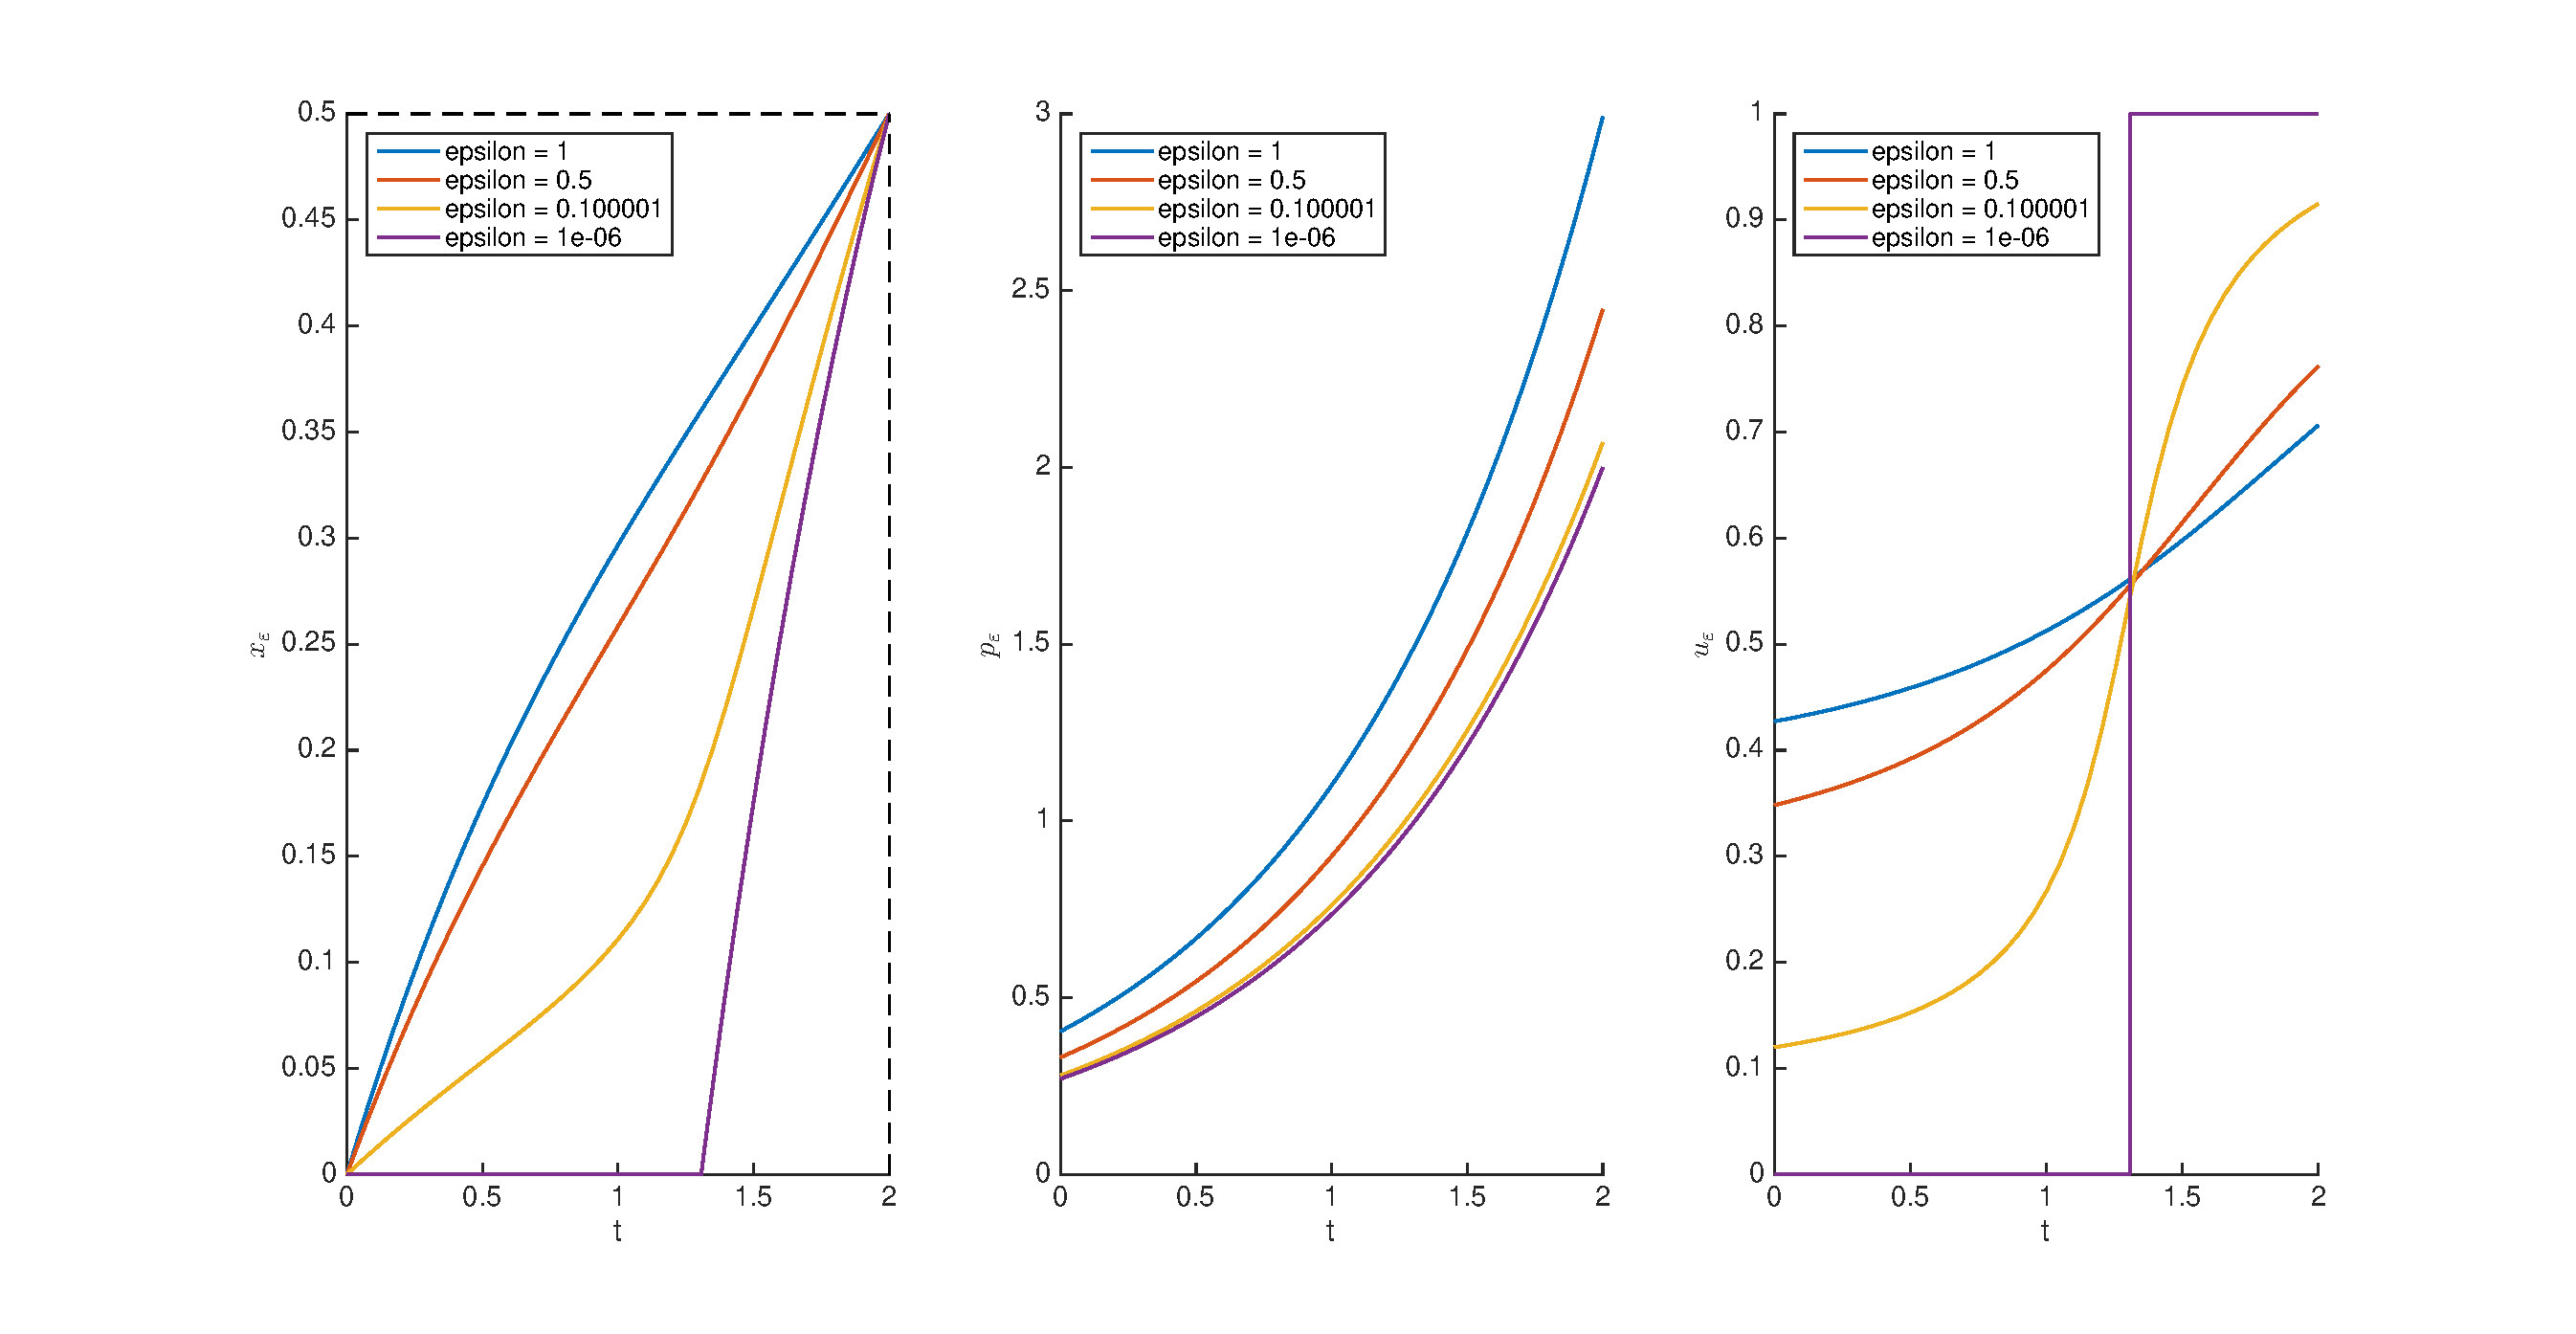
\includegraphics[width=0.99\textwidth]{results_tests_continuation}
    \end{center}
    \vspace{-3em}
    \caption{Figure 2 apr\`es ex\'ecution du fichier \cmd{sujet3\_continuation/main.m}.}
    \label{fig:results_tests_continuation}
\end{figure}

\begin{myExercice} Continuation discr\`ete sur le param\`etre $\veps$ et d\'etermination de la structure lorsque $\veps \to 0$.
    \begin{enumerate}
        \item Se rendre dans le r\'epertoire \cmd{sujet3\_continuation}.
        \item Impl\'ementer dans le r\'epertoire \cmd{lib} les fonctions \cmd{control}, \cmd{dcontrol}, \cmd{hvfun}, \cmd{dhvfun}, 
            \cmd{exphvfun}, \cmd{expdhvfun}, \cmd{sfun}, \cmd{sjac}, \cmd{finiteDiff} et \cmd{ssolve},
            associ\'ees au probl\`eme \eqref{eq:ocpBangReg} (voir \cmd{sujet2\_jacobienne/partie2/lib}).
        \item Compl\'eter le fichier \cmd{expcost.m} permettant de calculer la valeur du crit\`ere.
        \item Jouer sur les param\`etres (dans le fichier \cmd{main.m}) de la m\'ethode \cmd{lib/continuation} (voir \cmd{>> help continuation})
            et ex\'ecuter le script \cmd{main.m} pour retrouver les r\'esultats des figures
            \ref{fig:results_tests_continuation_1} et \ref{fig:results_tests_continuation}.
    \end{enumerate}
\end{myExercice}

\begin{myremark}
    On note $\arc_+$ un arc tel que $u(\cdot) \equiv +1$ tout au long de l'arc, $\arc_-$ si $u(\cdot) \equiv -1$ et $\arc_0$ si $u(\cdot) \equiv 0$.
    On note $\arc_1 \arc_2$ un arc $\arc_1$ suivi d'un arc $\arc_2$.
\end{myremark}

\begin{myQuestion}
    \label{question:continuation}
    Donner en fonction de $\arc_+$, $\arc_-$ et/ou $\arc_0$, la structure de la BC-extr\'emale limite lorsque $\veps \to 0$ pour le probl\`eme
    \eqref{eq:ocpBangReg}.
\end{myQuestion}
